\documentclass[11pt,a4paper,final]{report}
\usepackage[utf8]{inputenc}
\usepackage{amsmath}
\usepackage{amsfonts}
\usepackage{amssymb}
\usepackage{graphicx}
\usepackage{color}
\definecolor{red}{rgb}{1, 0, 0}
\usepackage[final]{listings}
\usepackage{url}
\author{S. Shiraiwa}
\title{Petra-M: Physics Equation Translator for MFEM}
\begin{document}
\lstset{language=Python}
\maketitle
\tableofcontents
\newpage

\chapter{Introduction}
Petra-M (Physics Equation Translator for MFEM) is a tool to build a finite element simulation model using MFEM. 
MFEM is a scalable finite element library built at LLNL. In MFEM,  a user has to fill the linear system matrix and the right hand side by adding  mfem::BilinearFormIntegrator and mfem::LinearFormIntegrator to mfem::BilinearForm and mfem::LinearForm.
While a variety of integrators are already defined in MFEM, translating a physics equation to a weakform and choosing a proper integrator for each case is an error-prone process. 
Another practical issue is to assign domain and boundary conditions for a particular element. A real world 3D geometry could contain several hundreds or even more surfaces and domains. Without an interactive interface, it is difficult to perform this step in a reliable manner.

Using Petra-M and $\pi$Scope, a user can build physics simulation model quickly and reliably.
Petra-M allows for creating a parametric geometry and mesh using GMSH Python API (and underling OpenCASCADE). 
Petra-M currently support the generic weakform interface where a user construct the physics equation directly specifying the mfem integrators, and the frequency domain Maxwell problems. low level engine is design to be flexible to expand in future.
In addition to the iterative solver interface in MFEM, Petra-M comes with interface to MUMPS direct solver

Goal of this report is to describe how Petra-M construct a linear system. An emphasis is on showing the weakform equation systems used for each physics module. Note that these equations are mostly well established and found in various literature, and therefore, providing the detailed derivation is not the point of this report. 

\textcolor{red}{We need to discuss several other things here, including 
client Server model, introduction of  NameSpace concept, time dependent solvers
}

\chapter{Preparing simulation model}
In this chapter, we discuss the interfaceo launch Petra-M in $\pi$Scope, 
\section{Starting Petra-M in  $\pi$Scope}

\section{Petra-M Model tree}
The simulation model in Petra-M is defined using Model Tree. MFEM viewer

\section{Linear System Structure}
Need to discusss,,,,Mesh space, FESpace variable, Auxiliary variable

\section{Namespace and Coefficients}
Using it for material property and selection index.
\subsection{Namespac (NS) and Dataset associated to NS}
Namespace (GUI uses NS in brief) is the concept to define the variable/functions which is local to the physics model. 
A user can use the variable defined the namespace as a parameter in physics setting. 

Dataset is a special model tree object, which holds the set of data. 
Each namespace is linked with one Dataset, and whena namespace is compiled the data stored in the Dataset is loaded at the beginning. 

Since the Dataset is a tree object, the data recorded in Dagaset  is saved to file whe the project is saved, and automatically loaded when the project file is opened.
Note that because of this behavior, Dataset can store only the pickable data. 

All Petra-M model treat has a default namespace, called global\_ns, and Dataset, called global\_data.

\subsection{Variable}
Petra-M has two different mechanism for specifying the coefficient which appears in a weakform formulation. One is Variable, discussed in the section.
Variable is a user defined function in Namespace, which is flagged using Variable decorator.
You can use the decorated Python fuction as s a functional coefficient.
When executing the simulation model, this decorate tells Petra-M to convert the function to a MFEM coefficient. 

\begin{minipage}[c]{0.95\textwidth}
\begin{lstlisting}[caption={A user defined generic preconditioner},captionpos=b, frame=single, label={function1}]

from petram.helper.variables import variable

@variable.float()

@variable.array(complex = False, shape=(3,3), \
               dependency=['vhts1', 's'])
def func(x, y, z, vhts1=None, s=None):

     # compute your material
     return np.array([[1,0,0], [0,1,0], [0,0,1]])

\end{lstlisting}
 \end{minipage}
 
\subsection{Coefficient}
Another mechanism is called Coefficient. 
In this approach, a user write a fucntion which returns MFEM coefficient. 

MFEM has a mechanism to define a complicate coefficient defined by atithmetic operation between more primitive coefficient. 
A user can writegenerate a MFEM coeffeicient using such compuond coefficients

Although it is more cumbersome to define the functinal coefficient this way, the resultant model can run faster because MFEM can avoid the overhead of calling Python function when assembling the forms.

The real advantage of this approach comes when a user write his/her own coefficeint in C++ and provide it as a Petra-M extension.  


\begin{minipage}[c]{0.95\textwidth}
\begin{lstlisting}[caption={A user defined generic preconditioner},captionpos=b, frame=single, label={function1}]

from petram.helper.variables import coefficient
@coefficient.array(shape=(3,3))
def three_one_one():
    value = np.diag((-3.,1.,1.))   
    coeff1 = mfem.MatrixConstantCoefficient(value)
    return coeff1

\end{lstlisting}
 \end{minipage}
 
\section{Auxiliary Variable and Operator}
\subsection{Operator}
\subsubsection{identity}            
\subsubsection{integral}
\subsubsection{projection}
\subsubsection{deltam}
\subsubsection{deltam}
deltam operator is an extention of delta operator. Deltam operator has a following argument interface.


Using it for material property and selection index.
\chapter{Geometry}

\chapter{Mesh}

\section{MFEM mesh}
FEM mesh is specified under MFEMMesh section in MESH section. Model objects under MFEMMesh
Mesh Operation Petra-M

\subsection{MeshFile}
MeshFile specify the mesh file used in the simulation. Note that when the path is left blank, Petra-M is going to use
a mesh file generated by using our GMSH mesh generator interface (discussed in Sec. \ref{GMSH_Mesh})

\begin{figure}
\centering
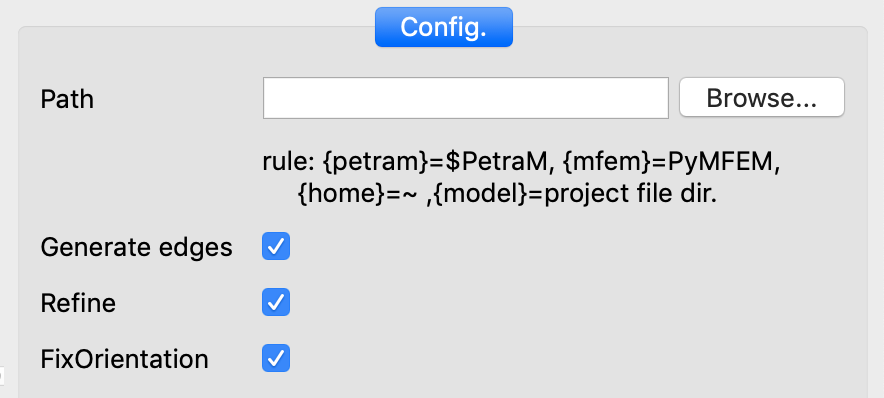
\includegraphics[width=0.75\columnwidth]{figures/mesh_file_gui.png} 
\caption{ Mesh file interface}\label{mesh_file}
\end{figure}


\subsection{Simple Mesh Generator}
We support generating a (very) simple mesh geometry directly as an MFEM mesh object. 
This mode is meant for a generating a simple mesh in quick for testing purpose.
Currently, it produces 1D linear mesh, 2D box meshed by rectangles and 3D box meshed
by hexahedra (more specifically rectangular cuboids). 
Note that in panels shown in Fig.\,\ref{simple_mesh}, we can put array in Length and Number of 
segment so that it generate multi-domain mesh. 

\begin{figure}
\centering
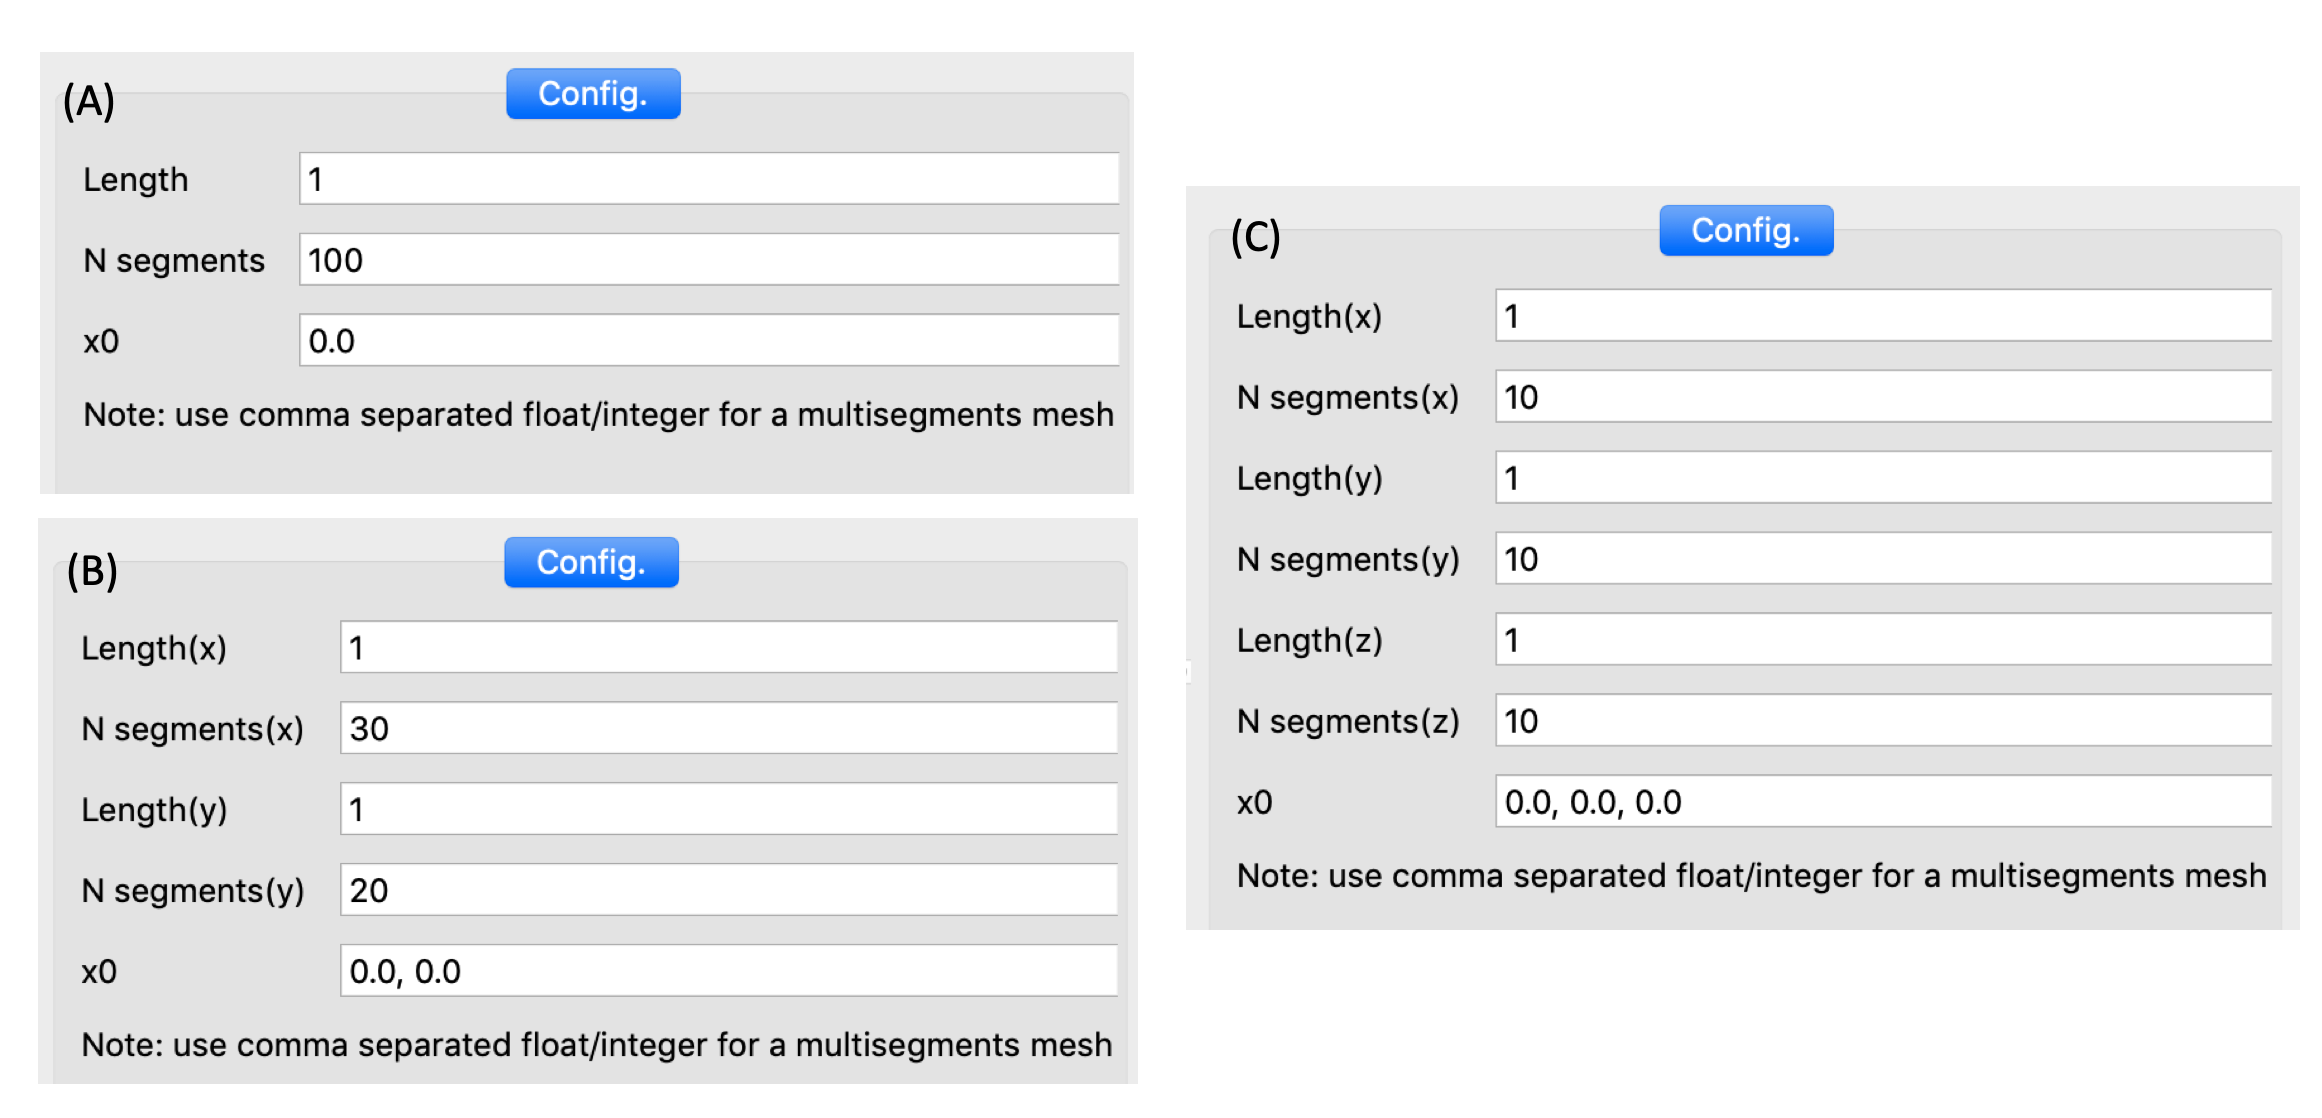
\includegraphics[width=0.95\columnwidth]{figures/simple_mesh_gui.png} 
\caption{ Simple Mesh Generator Panel for (A) 1D, (B) 2D, and (C) 3D mesh }\label{simple_mesh}
\end{figure}

\subsection{MeshOperation}
Petra-M allows to manipulate mesh. Currently, it allows UniformRefinement and DomainRefinement. 

\section{Mesh generator using GMSH}
\label{GMSH_Mesh}

\chapter{Physics}
\section{WeakForm(WF)}
\section{CoefficientForm(Coeff)}
\subsection{2D static (Coeff2D)}
This module solves the following equation in 2D (x, y) domain.
  \begin{align}
   \nabla (\mathbf{c} \nabla u + \mathbf{p}u + \mathbf{r}) + \mathbf{q} \cdot \nabla u + au - f = 0 
  \\  
  u = u_{0} \,\,\,on\,\,\,\partial \Omega_{1}
  \\
 \mathbf{n}\cdot (\mathbf{c} \nabla u + \mathbf{p}u + \mathbf{r}) = hu + g,\,\,on\,\,\,\partial \Omega_{2}
  \end{align}
  
 

 
  \subsection{2D time-dependent (Coeff2Dt)}
  \begin{align}
  m\frac{\partial^2 u}{\partial t^2} +   d\frac{\partial u}{\partial t} + \nabla (\mathbf{c} \nabla u + \mathbf{p}u + \mathbf{r}) + \mathbf{q} \cdot \nabla u + au - f = 0, 
  \\  
  u = u_{0} \,\,\,on\,\,\,\partial \Omega_{1},
  \\
 \mathbf{n}\cdot (\mathbf{c} \nabla u + \mathbf{p}u + \mathbf{r}) = hu + g,\,\,on\,\,\,\partial \Omega_{2},
  \end{align}
where m is the mass coefficient, d is the damping coefficient, c is the diffusion coefficient, p is the conservative flux convection coefficient. q is the convection coefficient,  a is the absorption coefficient, r is the conservative flux source term, and f is the source term.

 \subsection{Weakform}
  Multipling a test funcion $v$ from the left and integrating it over the computation domain,  we can transform the terms in the previous 2nd order PDE as follows.
  \begin{equation}
 \int v \nabla (\mathbf{c} \cdot \nabla u) = (\nabla v,\mathbf{c} \cdot \nabla u) - \langle v, \mathbf{c} \cdot \frac{\partial u}{\partial \mathbf{n}} \rangle
  \end{equation}
  
  a u + gamma) 
              + beta (grad u) + a u - f = 0

  On domain boundary
     n ( c grad u + alpha u - gamma) + q u = g - h$^t$ mu
       or 
     u = u0  

    m, d, a, f, g and h: scalar
    alpha, beta and gamma : vector
    c  : matrix (dim (space) $^2$)

    If all coefficients are independent from u, ux,
    the system is linear.

    BC
     Zero Flux : 
        n ( c grad u + alpha u - gamma) = 0
     Flux: 
        n ( c grad u + alpha u - gamma) = - g + q u
     Dirichlet Boundary Condition
        u = u0

  Weakform integrators:
    domain integral
       c     -->  c (grad u, grad v)     bi
       alpha -->  alpha * (u, grad v)    bi
       gamma -->  gamma * grad v         li
       beta  -->  beta * (grad u, v)     bi
       f     -->  (f, v)                 bi
    surface integral
       c     -->   n dot c (grad u, v)   bi
       alpha -->   n dot alpha  (u v)    bi
       gamma -->   n dot gamma   v       li
 
    surface integral can be replaced by (g - qu, v)
        
  Domain:   
     Coeff2D          : tensor dielectric

  Boundary:
     Coeff2D-Zero     : zero essential (default)
     Coeff2D-Esse     : general essential

'''
\section{Radio Frequency (EM)}

We employ $\exp{(-\omega t)}$ for time dependence. Then, from the Maxwell's equations, it follows,
\begin{equation}
\nabla \times \frac{1}{\mu_0} \nabla \times \mathbf{E} - (\omega^2 \epsilon + i \omega \sigma) \mathbf{E} = i \omega \mathbf{J}_{\rm ext}
\end{equation}

\subsection{3D frequency domain(EM3D)}
\subsubsection{Weakform of the Maxwell's equation}
This module uses the Cartesian coordinate system (x, y, z), and solves the following weakform of Maxwell equations. 
 \begin{align}
(\nabla \times \mathbf{F},  \frac{1}{\mu}\nabla  \times  \mathbf{E})
 - (\mathbf{F},  (\omega^2 \epsilon+ i \omega \sigma)  \mathbf{E}) 
 +  \langle \mathbf{F},  \mathbf{Q} \rangle 
 \notag \\
 - \gamma \langle  \mathbf{F}, \mathbf{n} \times \mathbf{n} \times  \mathbf{E}\rangle = i \omega (\mathbf{F}, \mathbf{J}_{\rm ext} ) ,
\label{em3d_weak} \\
\label{em3d_weakBC} 
 \mathbf{n} \times (\frac{1}{\mu} \nabla \times \mathbf{E}) + \gamma \mathbf{n} \times \mathbf{n} \times  \mathbf{E} = Q\,\,\,on\,\,\,\partial \Omega_{2}
 \end{align}
  where $(A , B)$ is the domain integral ($\int_{\Omega} AB dxdydz$) and $\langle A, B \rangle $ is the boundary integral ($\int_{\partial \Omega_{2}} ABdxdydz$). 
 
 \subsubsection{Anisotropic media}
 
 \subsubsection{External current source}
 
 \subsubsection{PMC (perfect magnetic conductor)}
 This BC forces $H_t$ = 0. This is the natural boundary condition in which $\gamma$ and $\mathbf{Q}$ are zeroed in Eq.~\ref{em3d_weakBC}.
 
 \subsubsection{PEC (perfect electric conductor/electric field BC}
 This BC forces $E_t$ = 0. This is a special case of essential BC.
 
 \subsubsection{Surface Current}
  
 \subsubsection{Port}
 Port can be used  on the boundary $\partial\Omega$, where the mode profile ($\mathbf{E}_{\rm mode}$ and $\mathbf{H}_{\rm mode}$) and the amplitude incoming mode ($A_{\rm inc}$) is known. The outgoing wave amplitude ($A_{\rm out}$) is not known and is solved as a part of equation. We use $\gamma=0$ and $\frac{1}{\mu}\nabla\times\mathbf{E}=i \omega \mathbf{H}$ in Eq.~\ref{em3d_weak} and obtain a linear system in the block matrix from,
\begin{equation}
\label{port_BC_blockmatrix}
 \begin{bmatrix}
 \mathbf{S}   & -\mathbf{N} \\
\mathbf{M}^t & 1\\
\end{bmatrix}
 \begin{bmatrix}
 \mathbf{x} \\
A_{\rm out}\\
\end{bmatrix}
=
 \begin{bmatrix}
A_{\rm inc} \mathbf{N}     \\
0 \\
\end{bmatrix},
 \end{equation}
where $\mathbf{N}$ is the linearform to impose  $\mathbf{H}_{\rm mode}$ using Eq.~\ref{em3d_weakBC} and is written as
\begin{equation}
\mathbf{N} = \langle \mathbf{F}, i \omega \mathbf{n} \times \mathbf{H}\rangle 
 \end{equation}
 
$\mathbf{M}^t$ is the weight to extract the mode amplitude from the solution vector $\mathbf{x}$. In the continuous form, it corresponds to the following 
\begin{equation}
\int \mathbf{E} \cdot \mathbf{E}_{\rm mode} \partial\Omega/\int \mathbf{E}_{\rm mode}  \cdot \mathbf{E}_{\rm mode} \partial\Omega
\end{equation}

In order to define $\mathbf{M}^t$ in the discrete space , we first the vector representation of $\mathbf{E}_{\rm mode}$ in the H(curl) space. This can be done by projecting the coefficient to GridFunction, and we note it as $\mathbf{E}_{\rm gf}$. Then $\mathbf{M}$ is given by
\begin{equation}
\mathbf{M} = \langle \mathbf{F}, \mathbf{E_{\rm mode}} \rangle / \langle \mathbf{F}, \mathbf{E}_{\rm mode} \rangle \cdot \mathbf{E}_{\rm gf},
 \end{equation}
where the dot product is computed between the second linearform and $\mathbf{E}_{\rm gf}$.

Note that the current implementation assumes that there is only one out-going mode. If the geometry allows to sustain multiple modes, we needs to expand Eq.~\ref{port_BC_blockmatrix} to include multiple modes. 

For the rectangular waveguide and coax port, we normalize the mode amplitude in such a way that the time averaged  incoming wave power is equal to 1[W]. For the coax (TEM) case, the following mode profiles are used.

 \begin{align}
E_{\rm mode} = A_{\rm n} \frac{\mathbf{r}}{r} \exp(kz)
\\
i \omega H_{\rm mode} = A_{\rm n} \omega \sqrt{\frac{\epsilon_{\rm 0}\epsilon_{\rm r}}{\mu_{\rm r}\mu_{\rm 0}}} \frac{\mathbf{r}}{r} \exp(kz)
\\
 A_{\rm n}^2 = \frac{1}{\pi \ln{(b/a)}} \sqrt{\frac{\mu_{\rm r}\mu_{\rm 0}}{\epsilon_{\rm 0}\epsilon_{\rm r}}}
\end{align}

For the waveguide (TE) case, the following mode profiles are used.
(...do be documented...)

Note that we define Poyx, Poyy, and Poyz (x, y and z components of the Poynting vector) as $E \times \overline{B}$, which is twice bigger than the time averaged power flux.

 \subsubsection{Surface Impedance}
 
This BC is to model a surface to which the RF wave penetrates only a short depth (a.k.a. skin depth, $\delta$), where $\delta$ is given by 
\begin{equation} 
\delta = \sqrt{\frac{2}{\omega \sigma \mu}}.
\end{equation}

On such a surface, the impedance (the ratio between E and H) is given as
\begin{equation}
\frac{E_{\rm x}}{H_{\rm y}} = \sqrt{\frac{i \omega \mu}{\sigma + i \omega \epsilon}} \sim \frac{1+i}{2} \omega \mu \delta
\end{equation}

Eq.\,\ref{em3d_weakBC} is viewed to define  the ratio between the tangential components of E and H, and the above relationship can be directly implemented. In general, we use the impedance $Z(\omega)$ 
\begin{equation}
\mathbf{n} \times \mathbf{n} \times \mathbf{E} + Z(\omega) \mathbf{n} \times \mathbf{H} = 0
\end{equation}
 and express $\gamma$ in Eq.\,\ref{em3d_weakBC} using $Z(\omega)$, while $\mathbf{Q}$ is zero. 
 
 \subsubsection{Periodic (Floquet-Bloch) BC}
 
 
\subsection{Axisymmetric frequency domain(EM2Da)}
\subsubsection{Weakform of the Maxwell's equation}
This module uses the cylindrical coordinate system (r,  $\phi$, z). Physics quantities are supposed to have a periodic dependence to 
$\phi$ direction ($\sim e^{m \phi}$), where $m$ is the out-of-plane mode number. First, we write the curl operator in the following form

 \begin{align}
 \nabla \times E = &(\frac{im}{r} E_{\rm z} - \frac{\partial E_{\phi}}{\partial z})\mathbf{e}_{\rm r} +
( \frac{\partial E_{\rm r}}{\partial z} - \frac{\partial E_{\rm z}}{\partial r})\mathbf{e}_{\rm \phi}+
 (\frac{1}{r}\frac{\partial }{\partial r}(r E_{\phi}) - \frac{im}{r} E_{\rm r} )\mathbf{e}_{\rm z} 
 \notag \\ 
 = &\nabla_{t} \times \mathbf{E}_{\rm t} + \frac{\mathbf{e}_{\rm \phi}}{r} \times (im \mathbf{E}_{\rm t} - \nabla_{\rm t} (rE_{\rm \phi}) ),
 \end{align}
 where $\mathbf{E}_{\rm t} = (E_{\rm r}, E_{\rm z})$ and  $\nabla_{t} = (\frac{\partial }{\partial r}, \frac{\partial }{\partial z}$) are 2D vectors on $r$, $z$ plane.
 
Then, we exapned the weakform for Maxwell equations (Eq.\,\ref{em3d_weak}) using $\mathbf{E}_{\rm t}$, $E_{\phi}$, and $\nabla_{t}$ so that a direct one-by-one connection to mfem::LinearFormIntegrator and mfem::BilinearFormIntegrator becomes clear.
For a scolar $\mu$, $\epsilon$, and $\sigma$, it can be written as \textcolor{red}{correct this expression. Jacobian should be inside the blacket}
 \begin{align}
r(\nabla_{\rm t} \times \mathbf{F}_{\rm t},  \frac{1}{\mu}\nabla_{\rm t}  \times & \mathbf{E}_{\rm t}) 
+\frac{1}{r} m^2(\mathbf{F}_{\rm t}, \frac{1}{\mu}\mathbf{E}_{\rm t})
+ \frac{1}{r} (\nabla_{\rm t} (rF_{\rm \phi}), \frac{1}{\mu}\nabla_{\rm t} (rE_{\rm \phi}))
 \notag \\
+& \frac{1}{r} (im \mathbf{F}_{\rm t}, \frac{1}{\mu}\nabla_{\rm t} (rE_{\rm \phi}))
- \frac{1}{r} (\nabla_{\rm t} (rF_{\rm \phi}), \frac{im}{\mu} \mathbf{E}_{\rm t})
 \notag \\
 -& (\omega^2 \epsilon+ i \omega \sigma) ( r( \mathbf{F}_{\rm t}, \mathbf{E}_{\rm t}) + \frac{1}{r}(rF_{\rm \phi}, rE_{\rm \phi})) 
 \notag \\
 +& r \langle \mathbf{F}_{\rm t},  \mathbf{Q}_{\rm t} \rangle + \langle rF_{\rm \phi}, Q_{\rm phi} \rangle -r \gamma \langle \mathbf{F}_{\rm t}, \mathbf{E}_{\rm t} \rangle
 \notag \\
 =& i \omega r ( \mathbf{F}_{\rm t}, \mathbf{J}_{\rm t} ) + i \omega ( rF_{\rm \phi}, J_{\rm \phi} ), \label{em2da_weak}
 \end{align}
 where $(A , B)$ is the domain integral ($\int_{\Omega} AB drdz$) and $\langle A, B \rangle $ is the boundary integral ($\int_{\partial \Omega} ABds$). The module uses the H(curl) element for $\mathbf{E}_{\rm t}$ and the H1 element for $rE_{\phi}$. Note that the integration does not consider $2 \pi r$ and $r$ is included in the coefficient of the linear/bilinear forms. 
 
 \subsubsection{Anisotropic media}
 
In the mass integrator, we expand $\epsilon$ and $\sigma$ into the following block. Currently anisotropc $\mu$ is not supported.

 \begin{equation}
 \left[ {\begin{array}{*{20}c}
\mathbf{F}_{\rm t}  & rF_{\rm \phi}\\
\end{array}}\right]
\left[ {\begin{array}{*{20}c}
\mathbf{\epsilon}_{\perp \perp}  & \frac{\mathbf{\epsilon}_{\perp \parallel}}{r}\\
\frac{\mathbf{\epsilon}_{\parallel \perp}}{r} & \frac{\mathbf{\epsilon}_{\parallel \parallel}}{r^2}\\
\end{array}}\right]
 \left[ {\begin{array}{*{20}c}
\mathbf{E}_{\rm t}  \\
rE_{\rm \phi}\\
\end{array}}\right]
\label{em2da_anisotropic}
\end{equation}

 \subsubsection{External current source}
 This domain condition is implemented using the last line of Eq.\,\ref{em2da_weak}. 
 
 \subsubsection{PMC (perfect magnetic conductor)}
 
 \subsubsection{PEC (perfect electric conductor/electric field BC}
  
\subsection{2D frequency domain(EM2D)}
\subsubsection{Weakform}
in this mode, we solve the Maxwell equation in 2D (xy) space, assuming that the RF electric field has the form of $\mathbf{E}(x, y) \exp{(ikz)}$. 
In this geometry, the curl operator is expanded as follows,

 \begin{align}
 \nabla \times E = &(\frac{\partial E_{z}}{\partial y}- ik E_{\rm y} )\mathbf{e}_{\rm x} +
( -\frac{\partial E_{\rm z}}{\partial x} + ik E_{\rm x})\mathbf{e}_{\rm \phi}+
( \frac{\partial E_{\rm y}}{\partial x} - \frac{\partial E_{\rm x}}{\partial y})\mathbf{e}_{\rm z} 
 \notag \\ 
 = &\nabla_{t} \times \mathbf{E}_{\rm t} + \mathbf{e}_{\rm z} \times (ik \mathbf{E}_{\rm t} - \nabla_{\rm t} E_{\rm z}) ),
 \end{align}

Correspondingly, the weakform can be written as follows for a scalar $\mu$, $\epsilon$,  and $\sigma$
\begin{align}
(\nabla_{\rm t} \times \mathbf{F}_{\rm t},  \frac{1}{\mu}\nabla_{\rm t}  \times & \mathbf{E}_{\rm t}) 
+  k^2(\mathbf{F}_{\rm t}, \frac{1}{\mu}\mathbf{E}_{\rm t})
+ (\nabla_{\rm t} (F_{\rm z}), \frac{1}{\mu}\nabla_{\rm t} (E_{\rm z}))
 \notag \\
+& (ik \mathbf{F}_{\rm t}, \frac{1}{\mu}\nabla_{\rm t} E_{\rm z})
- (\nabla_{\rm t} F_{\rm \phi}, \frac{ik}{\mu} \mathbf{E}_{\rm z})
 \notag \\
 -& (\omega^2 \epsilon+ i \omega \sigma) (  \mathbf{F}_{\rm t}, \mathbf{E}_{\rm t} + (F_{\rm z}, E_{\rm z})) 
 \notag \\
 +& \langle \mathbf{F}_{\rm t},  \mathbf{Q}_{\rm t} \rangle + \langle F_{\rm z}, Q_{\rm z} \rangle 
 - \gamma \langle \mathbf{F}_{\rm t}, \mathbf{E}_{\rm t} \rangle
 - \gamma \langle F_{\rm z}, E_{\rm z} \rangle
 \notag \\
 =& i \omega ( \mathbf{F}_{\rm t}, \mathbf{J}_{\rm t} ) + i \omega ( F_{\rm z}, J_{\rm z} ), \label{em2d_weak}
 \end{align}

Mass integrator for an anistropic $\epsilon$ and $\sigma$ can be written in a similar way as Eq.\,\ref{em2da_anisotropic}. 
Curl-Curl integrator is also treated in the same way. But xy-xy component of $1/\mu$ is replaced by the adjoint matrix, also note
that the off-diagonal block of magnetic permeability is not implemented, yet. 

 \begin{equation}
 \left[ {\begin{array}{*{20}c}
\mathbf{F}_{\rm t}  & F_{\rm z}\\
\end{array}}\right]
\left[ {\begin{array}{*{20}c}
\mathbf{\epsilon}_{\perp \perp}  & \mathbf{\epsilon}_{\perp \parallel}\\
\mathbf{\epsilon}_{\parallel \perp} & \mathbf{\epsilon}_{\parallel \parallel}\\
\end{array}}\right]
 \left[ {\begin{array}{*{20}c}
\mathbf{E}_{\rm t}  \\
E_{\rm z}\\
\end{array}}\right]
\label{em2d_anisotropic}
\end{equation}


\subsection{1D frequency domain(EM1D)}


\section{Thermal Modules}
\subsection{3D static (TH3Ds)}


\chapter{Linear system assembly}
\section{Mesh extension} 
\section{Name space}
\section{Matrix assembly}
\
\chapter{IntialValue}
\label{InitialValue}    

\chapter{Postprocess}
\label{Postprocess}       
\section{Derived Value}     
Create a new grid function and project expression.
Extended Mesh must be generated in the solve stage.

\section{DWC (direct wrapper call)}

\chapter{Solver}
\section{Organization of Solver Section}
In Petra-M project, Solver section defines how it solves the PDE systems defined in Physics section. 
We view solving multi-physics PDE system as a process of assembling and solving multiple linear systems in a given sequence. 
The structure of Solver section is designed to define such a sequence. 
Top level of Solver section consists from a set of SolveSteps (or its subclasses). 
Under SolveStep, Solver objects, such as StdSolver, TimeDependentSolvers are listed. 
Each Solver defines a linear solver used to solve a linear system. 
In this seciotn, we discuss the role of each layer. 

\section{SolveStep}
In Petra-M, one SolveStep corresponds to one linear block matrix structure. 
The regular SolveStep panel on the model editor looks like Fig. \ref{solve_step}.
The block structure is determined by giving the discrete space variables in the test (dual) and trial  (primal) vectors. 
If this box is left black, Petra-M chooses the trail space based on the physics model to be solved and use the same block structure for the test space, too.
Another important role of SolveStep is to define how to initialize the trial vector, and how to postprocess the solution.
Initialization is defined by choosing the prescription prepared in InitialValue section of model (discussed in Chapter \ref{InitialValue})
Similariy, Postprocess can be defined by choosing the prescription defined in Postprocess section of model tree (
Additionally, Petra-M provides are an approach to post-process the solution vector without using the panels in model tree. This is called DWC (direct wrapper call).
DWC is meant for more low-level access to the solution (mfem GridFunction). 
Both approach are discussed in Chapter \ref{Postprocess}). 

\begin{figure}
\centering
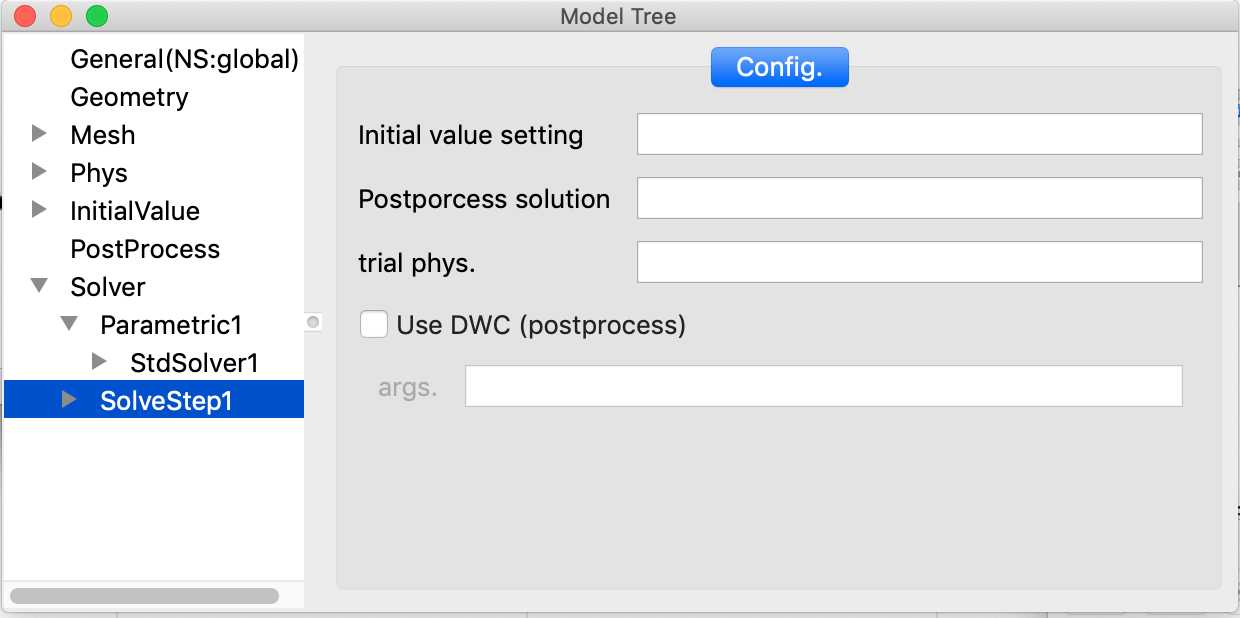
\includegraphics[width=0.95\columnwidth]{figures/solve_step.png} 
\caption{  }\label{solve_step}
\end{figure}


\subsection{Parametric Solver}
Parametric Solver (Fig. \ref{parametric_scan}) is a special kind of SolveStep, which allows to repeat the StdSolver run for a different value sets in   in NameSpace variables. 
Parametric Solver can run in two modes. In the first mode, the entire linear system is filled for every parameter set.
In the second mode, the only right hand side of equation is refilled. When using a direct solver supporting the multiple
right hand side, the second mode reuses the LU factorization. 
Scanner defines the parameter values used in the scan.  In the example shown in figure, Scan is the predefined parametric scanner (petram.solver.parametric\_scanner.py). 
This scanner defines the linear scan of parameters in multiple dimensions. 
In this case, it is setup to scan freq and ph for thee values and two values respectively. 
Scan takes the product of these two parameters and performs total 6 linear system solves.
List. \ref{parametric_scanner} shows details of how to give arguments to Scan.

\begin{minipage}[c]{0.95\textwidth}
\begin{lstlisting}[caption={Parametric Scanner},captionpos=b, frame=single, label={parametric_scanner}]
Scan("freq", [3e9, 4e9, 5e9])
Scan("freq", [3e9, 4e9, 5e9], "phase", [0, 90, 180])
Scan("freq", [3e9, 4e9, 5e9], "phase", [0, 90, 180], 
      product = False) #1D scan
Scan("freq", "phase", start = (3e9, 0), 
      stop = (5e9, 180), nstep = 3)  # 1D scan 
 Scan("freq", "phase", start = (3e9, 0), 
      stop = (5e9, 180),  nstep = (3,4)) # 2D scan 
\end{lstlisting}
\end{minipage}

\begin{figure}
\centering
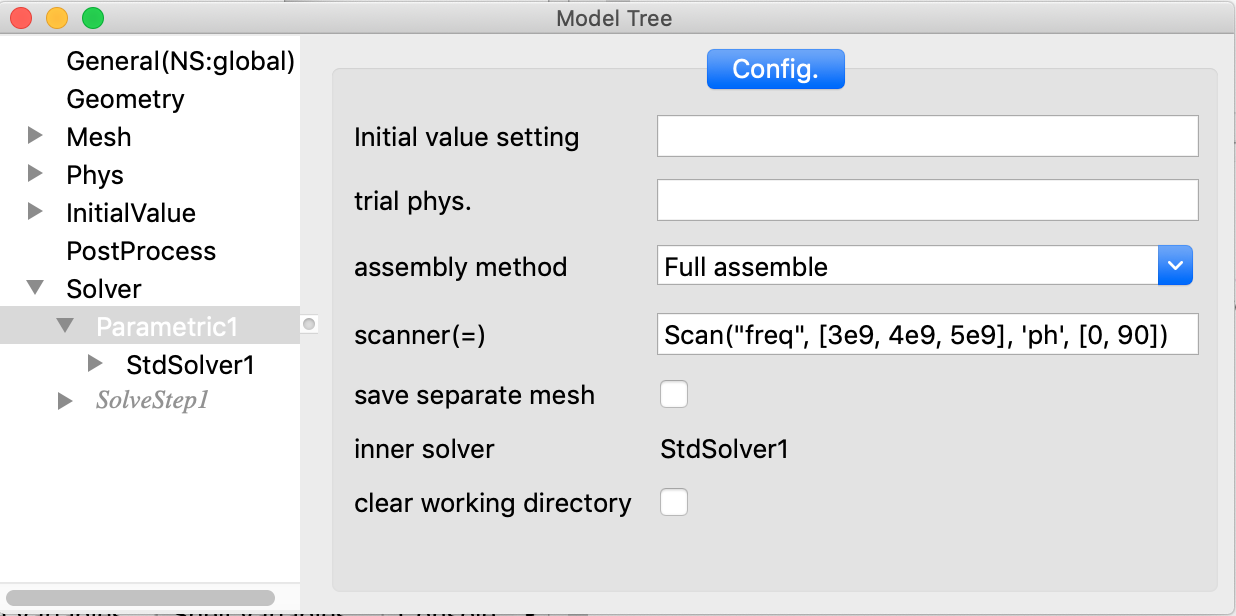
\includegraphics[width=0.95\columnwidth]{figures/parametric_scan.png} 
\caption{  }\label{parametric_scan}
\end{figure}

\section{Solver}

\section{LinearSolver}
\subsection{MUMPS}
MUMPS is a sparse direct solver (\url{http://mumps.enseeiht.fr}). Petra-M support MUMPS via the Petra\_MUMPS module. 

\subsection{Strumpack}
Supporting STRUMPACK is in progress.

\subsection{Iterative Solver}
\subsubsection{preconditioner}


\subsubsection{user defined preconditioner}
A user can also define his/her own preconditioner using python script.  This can be done in several levels, but all
uses the prc decorator to tell PetraM that a function in a script is to be used as a preconditioner object.

The first approach is to use $@$prc.block decoeator (Listing.\,\ref{prc1}). This is to define a preconditioner block element.  The defined element can be used either via a GUI discussed in the previous subsection or a user defined precontioner discussed below.  


A user can use $@$prc.blk\_diagonal and $@$prc.blk\_lowertriagular to define a diagonal and a lowertriangular precondiionter, respectively (Listing.\,\ref{prc2}).. In the decorated function, a user fill the preconditioner element using preconditioner blockblocks. Additionally, a user may create a complete precondtioner object using $@$prc.blk\_generic. In this case,SetOperator and Mult methods should be defined  by a user too.(Listing.\,\ref{prc3}). 

\begin{minipage}[c]{0.95\textwidth}
\begin{lstlisting}[caption={A user defined preconditioner block},captionpos=b, frame=single, label={prc1}]
@prc.block
def GS(**kwargs)
    prc = kwargs.pop('prc')
    blockname = kwargs.pop('blockname')
    mat = prc.get_diagoperator_by_name(blockname)
    if use_parallel:
        smoother = mfem.HypreSmoother(mat)
        ktype = getattr(mfem.HypreSmoother, "GS")
        smoother.SetType(ktype)
    else:
        smoother = mfem.GSSmoother(mat, 0)
        smoother.iterative_mode = False
    return smoother
\end{lstlisting}
\end{minipage}

\begin{minipage}[c]{0.95\textwidth}
\begin{lstlisting}[frame=single, caption={A user defined diag/lowertriangular preconditioner},captionpos=b, label={prc2}]
from petram.helper.preconditioners import prc
from petram.helper.preconditioners import GS as GSg
@prc.blk_diagonal
def D(p, g, *args, **kwargs):
    '''
    definition of block diagonal preconditioner
    p is a preconditioner object. In this case,
     mfem.BlockDiagonalPreconditioner
    g is a preconditioner generator object carrying 
    the information of matrix.
    This example set GS for unknown v.  
    '''
    GSg.set_param(g, "v")
    gs = GSg() #instatiate a block
    k = g.get_row_by_name("v")
    p.SetDiagonalBlock(k, gs) # set to block
    return p
    
@prc.blk_lowertriagular
def prc_tri(p, **kwargs):
    '''
    definition of lower trianuglar preconditioner
    '''
    p.Mult(x, y)
\end{lstlisting}
\end{minipage}

\begin{minipage}[c]{0.95\textwidth}
\begin{lstlisting}[caption={A user defined generic preconditioner},captionpos=b, frame=single, label={prc3}]
@prc.blk_generic
def G(p, **kwargs):


@G.Mult
def Mult(p, x, y):
      '''
      contents of Mult method. 
      x is input, while y is output
      '''

@G.SetOperator
def SetOperator(p, opr):
      '''
      Update preconditioner using opr.
      '''
\end{lstlisting}
 \end{minipage}

\chapter{Visualization}
\section{Solution file structure}
\section{Plotting solution in $\pi$Scope}

\begin{figure}
\centering
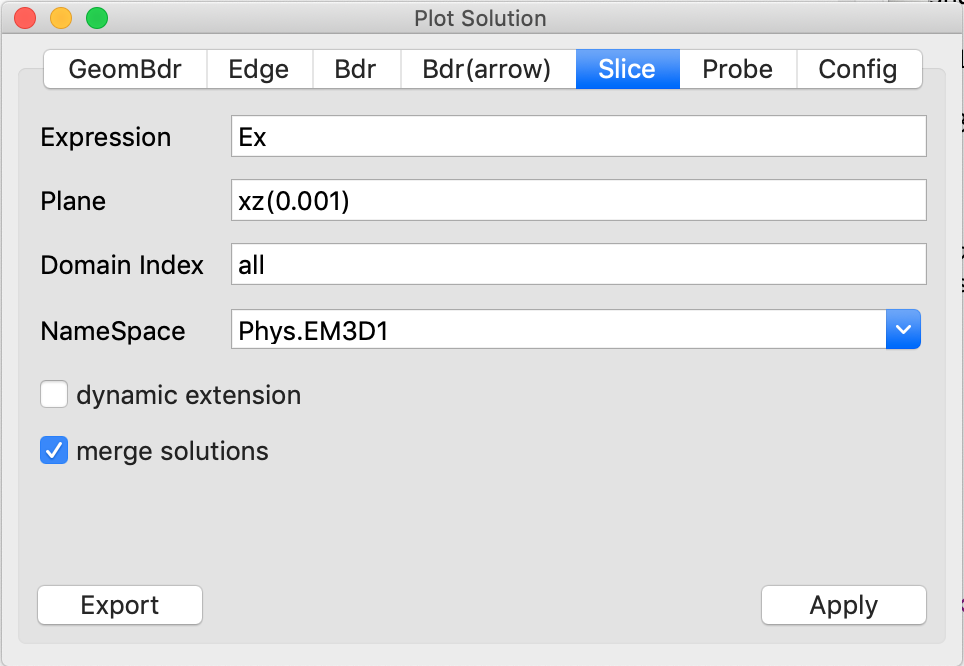
\includegraphics[width=0.95\columnwidth]{figures/slice_plot.png} 
\caption{ Plane can be defined "1, 0, 0. 0" , "xy", "xy(0.001)" }\label{parametric_scan}
\end{figure}


\chapter{Development}
\section{Source code organization}
\section{Extension}
PetraM\_Base\_ext

\section{Appendix}
\subsection{Release Histoery}

2018 08 24  The first public release version

\subsection{Revision Histoery}

2020. 06. 05: (In OCC) MergeFaces are introduced. This is because ShapeUpgrade does not allwasy connect surfaces. It appears when the normal is opposite, it does not consider two surfaces as a same domain. MergeFaces uses two boolean cut operation, and works only for the planner surfaces.
2020. 06. 05: (In OCC) Changed remove not to put back wire/shell when recursive is off. Instead. it put back edge and faces.

2017.


\end{document}